% Created by tikzDevice version 0.12.6 on 2025-01-17 13:26:13
% !TEX encoding = UTF-8 Unicode
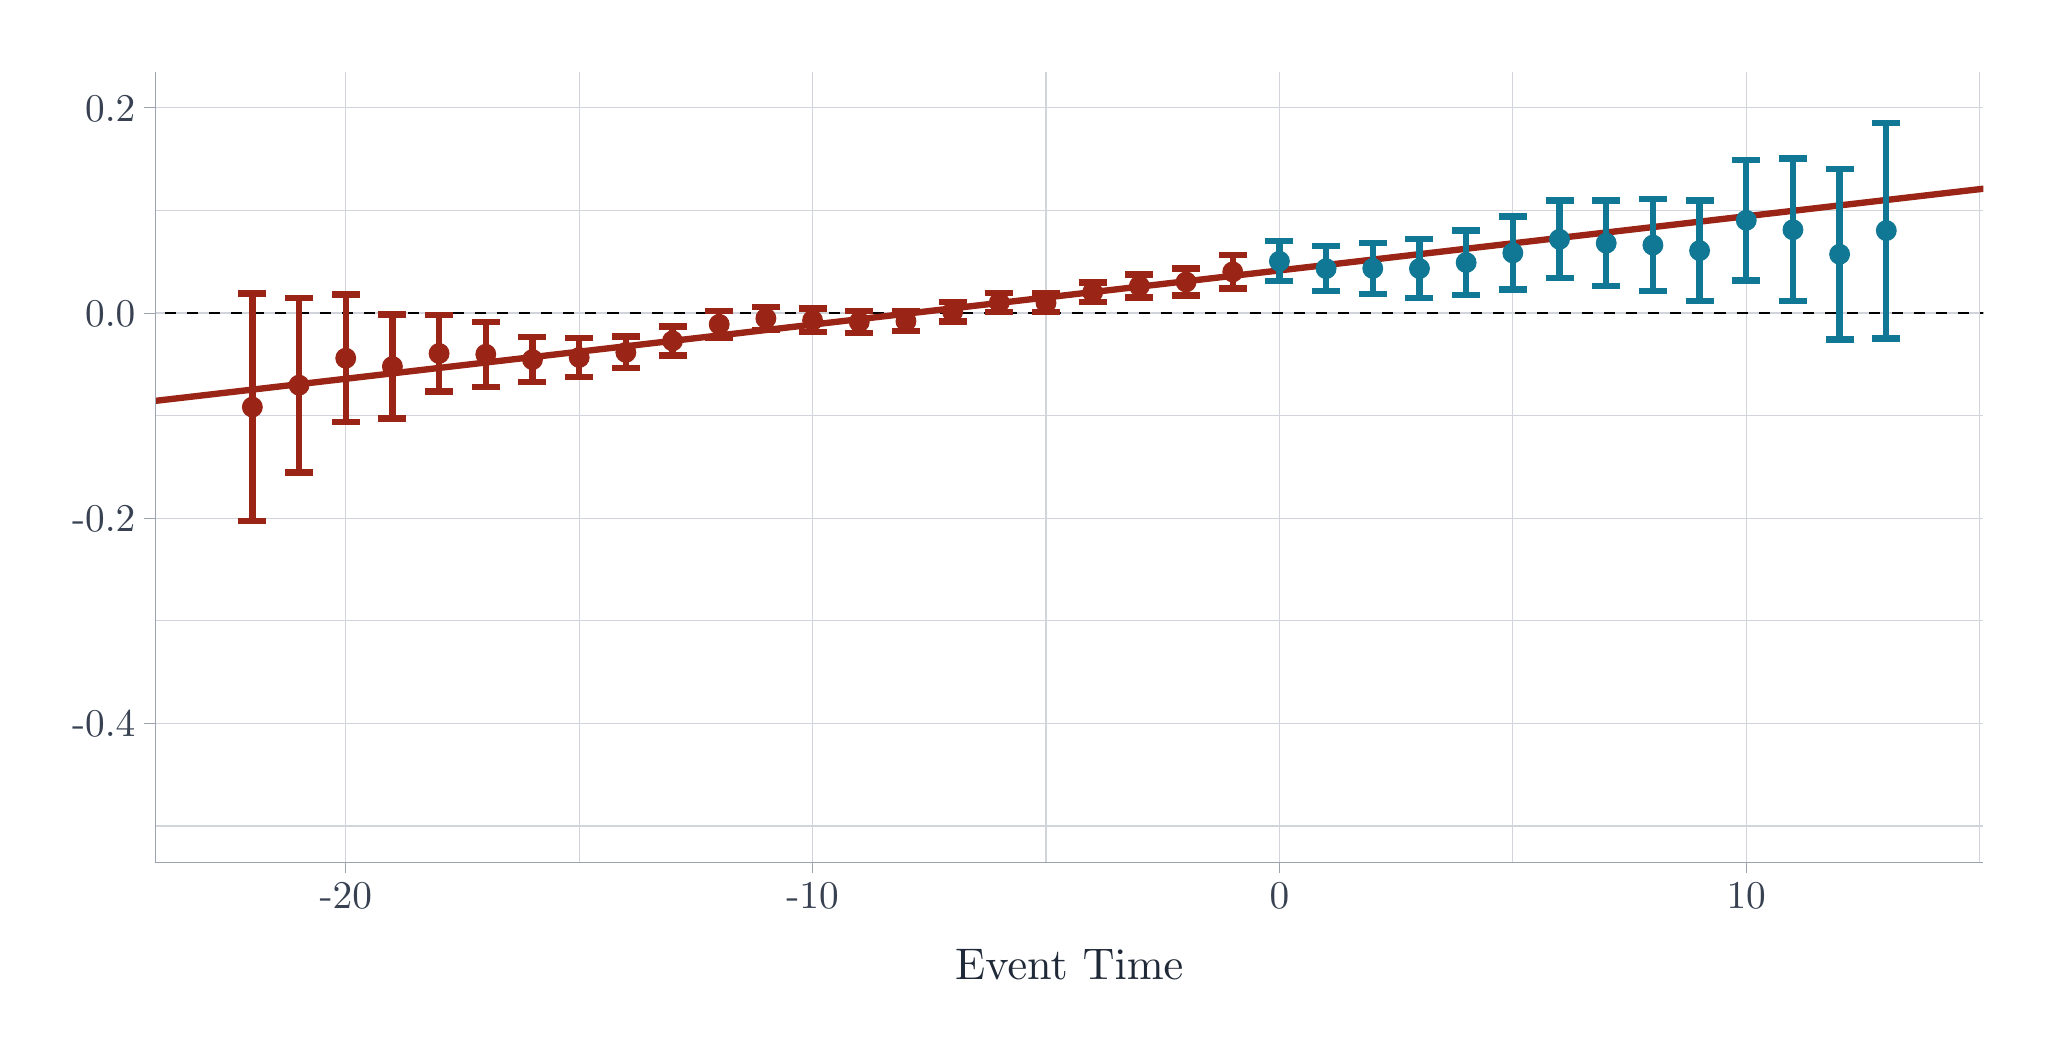
\begin{tikzpicture}[x=1pt,y=1pt]
\definecolor{fillColor}{RGB}{255,255,255}
\path[use as bounding box,fill=fillColor] (0,0) rectangle (722.70,361.35);
\begin{scope}
\path[clip] (  0.00,  0.00) rectangle (722.70,361.35);
\definecolor{drawColor}{RGB}{255,255,255}

\path[draw=drawColor,line width= 0.8pt,line join=round,line cap=round,fill=fillColor] (  0.00,  0.00) rectangle (722.70,361.35);
\end{scope}
\begin{scope}
\path[clip] ( 46.10, 59.89) rectangle (706.70,345.35);
\definecolor{drawColor}{RGB}{255,255,255}
\definecolor{fillColor}{RGB}{255,255,255}

\path[draw=drawColor,line width= 0.8pt,line join=round,line cap=round,fill=fillColor] ( 46.10, 59.89) rectangle (706.70,345.35);
\definecolor{drawColor}{RGB}{209,213,219}

\path[draw=drawColor,line width= 0.4pt,line join=round] ( 46.10, 72.86) --
	(706.70, 72.86);

\path[draw=drawColor,line width= 0.4pt,line join=round] ( 46.10,147.01) --
	(706.70,147.01);

\path[draw=drawColor,line width= 0.4pt,line join=round] ( 46.10,221.16) --
	(706.70,221.16);

\path[draw=drawColor,line width= 0.4pt,line join=round] ( 46.10,295.30) --
	(706.70,295.30);

\path[draw=drawColor,line width= 0.4pt,line join=round] (199.28, 59.89) --
	(199.28,345.35);

\path[draw=drawColor,line width= 0.4pt,line join=round] (367.97, 59.89) --
	(367.97,345.35);

\path[draw=drawColor,line width= 0.4pt,line join=round] (536.66, 59.89) --
	(536.66,345.35);

\path[draw=drawColor,line width= 0.4pt,line join=round] (705.35, 59.89) --
	(705.35,345.35);

\path[draw=drawColor,line width= 0.4pt,line join=round] ( 46.10,109.94) --
	(706.70,109.94);

\path[draw=drawColor,line width= 0.4pt,line join=round] ( 46.10,184.08) --
	(706.70,184.08);

\path[draw=drawColor,line width= 0.4pt,line join=round] ( 46.10,258.23) --
	(706.70,258.23);

\path[draw=drawColor,line width= 0.4pt,line join=round] ( 46.10,332.37) --
	(706.70,332.37);

\path[draw=drawColor,line width= 0.4pt,line join=round] (114.93, 59.89) --
	(114.93,345.35);

\path[draw=drawColor,line width= 0.4pt,line join=round] (283.62, 59.89) --
	(283.62,345.35);

\path[draw=drawColor,line width= 0.4pt,line join=round] (452.31, 59.89) --
	(452.31,345.35);

\path[draw=drawColor,line width= 0.4pt,line join=round] (621.00, 59.89) --
	(621.00,345.35);
\definecolor{drawColor}{RGB}{0,0,0}

\path[draw=drawColor,line width= 0.9pt,dash pattern=on 4pt off 4pt ,line join=round] (-614.49,258.23) -- (1367.30,258.23);
\definecolor{drawColor}{RGB}{154,36,21}

\path[draw=drawColor,line width= 2.3pt,line join=round] (-614.49,149.83) -- (1367.30,379.81);
\definecolor{fillColor}{RGB}{154,36,21}

\path[draw=drawColor,line width= 0.4pt,line join=round,line cap=round,fill=fillColor] ( 81.19,224.25) circle (  3.57);

\path[draw=drawColor,line width= 0.4pt,line join=round,line cap=round,fill=fillColor] ( 98.06,232.17) circle (  3.57);

\path[draw=drawColor,line width= 0.4pt,line join=round,line cap=round,fill=fillColor] (114.93,241.91) circle (  3.57);

\path[draw=drawColor,line width= 0.4pt,line join=round,line cap=round,fill=fillColor] (131.80,238.92) circle (  3.57);

\path[draw=drawColor,line width= 0.4pt,line join=round,line cap=round,fill=fillColor] (148.67,243.62) circle (  3.57);

\path[draw=drawColor,line width= 0.4pt,line join=round,line cap=round,fill=fillColor] (165.54,243.33) circle (  3.57);

\path[draw=drawColor,line width= 0.4pt,line join=round,line cap=round,fill=fillColor] (182.41,241.41) circle (  3.57);

\path[draw=drawColor,line width= 0.4pt,line join=round,line cap=round,fill=fillColor] (199.28,242.18) circle (  3.57);

\path[draw=drawColor,line width= 0.4pt,line join=round,line cap=round,fill=fillColor] (216.15,244.01) circle (  3.57);

\path[draw=drawColor,line width= 0.4pt,line join=round,line cap=round,fill=fillColor] (233.01,248.16) circle (  3.57);

\path[draw=drawColor,line width= 0.4pt,line join=round,line cap=round,fill=fillColor] (249.88,254.14) circle (  3.57);

\path[draw=drawColor,line width= 0.4pt,line join=round,line cap=round,fill=fillColor] (266.75,256.30) circle (  3.57);

\path[draw=drawColor,line width= 0.4pt,line join=round,line cap=round,fill=fillColor] (283.62,255.59) circle (  3.57);

\path[draw=drawColor,line width= 0.4pt,line join=round,line cap=round,fill=fillColor] (300.49,254.99) circle (  3.57);

\path[draw=drawColor,line width= 0.4pt,line join=round,line cap=round,fill=fillColor] (317.36,255.25) circle (  3.57);

\path[draw=drawColor,line width= 0.4pt,line join=round,line cap=round,fill=fillColor] (334.23,258.65) circle (  3.57);

\path[draw=drawColor,line width= 0.4pt,line join=round,line cap=round,fill=fillColor] (351.10,262.03) circle (  3.57);

\path[draw=drawColor,line width= 0.4pt,line join=round,line cap=round,fill=fillColor] (367.97,261.94) circle (  3.57);

\path[draw=drawColor,line width= 0.4pt,line join=round,line cap=round,fill=fillColor] (384.84,265.73) circle (  3.57);

\path[draw=drawColor,line width= 0.4pt,line join=round,line cap=round,fill=fillColor] (401.71,268.00) circle (  3.57);

\path[draw=drawColor,line width= 0.4pt,line join=round,line cap=round,fill=fillColor] (418.58,269.46) circle (  3.57);

\path[draw=drawColor,line width= 0.4pt,line join=round,line cap=round,fill=fillColor] (435.44,273.09) circle (  3.57);
\definecolor{drawColor}{RGB}{16,120,149}
\definecolor{fillColor}{RGB}{16,120,149}

\path[draw=drawColor,line width= 0.4pt,line join=round,line cap=round,fill=fillColor] (452.31,276.95) circle (  3.57);

\path[draw=drawColor,line width= 0.4pt,line join=round,line cap=round,fill=fillColor] (469.18,274.27) circle (  3.57);

\path[draw=drawColor,line width= 0.4pt,line join=round,line cap=round,fill=fillColor] (486.05,274.35) circle (  3.57);

\path[draw=drawColor,line width= 0.4pt,line join=round,line cap=round,fill=fillColor] (502.92,274.30) circle (  3.57);

\path[draw=drawColor,line width= 0.4pt,line join=round,line cap=round,fill=fillColor] (519.79,276.48) circle (  3.57);

\path[draw=drawColor,line width= 0.4pt,line join=round,line cap=round,fill=fillColor] (536.66,279.95) circle (  3.57);

\path[draw=drawColor,line width= 0.4pt,line join=round,line cap=round,fill=fillColor] (553.53,284.88) circle (  3.57);

\path[draw=drawColor,line width= 0.4pt,line join=round,line cap=round,fill=fillColor] (570.40,283.48) circle (  3.57);

\path[draw=drawColor,line width= 0.4pt,line join=round,line cap=round,fill=fillColor] (587.27,282.79) circle (  3.57);

\path[draw=drawColor,line width= 0.4pt,line join=round,line cap=round,fill=fillColor] (604.14,280.78) circle (  3.57);

\path[draw=drawColor,line width= 0.4pt,line join=round,line cap=round,fill=fillColor] (621.00,291.74) circle (  3.57);

\path[draw=drawColor,line width= 0.4pt,line join=round,line cap=round,fill=fillColor] (637.87,288.32) circle (  3.57);

\path[draw=drawColor,line width= 0.4pt,line join=round,line cap=round,fill=fillColor] (654.74,279.48) circle (  3.57);

\path[draw=drawColor,line width= 0.4pt,line join=round,line cap=round,fill=fillColor] (671.61,288.02) circle (  3.57);
\definecolor{drawColor}{RGB}{154,36,21}

\path[draw=drawColor,line width= 2.3pt,line join=round] ( 76.13,265.34) --
	( 86.25,265.34);

\path[draw=drawColor,line width= 2.3pt,line join=round] ( 81.19,265.34) --
	( 81.19,183.15);

\path[draw=drawColor,line width= 2.3pt,line join=round] ( 76.13,183.15) --
	( 86.25,183.15);

\path[draw=drawColor,line width= 2.3pt,line join=round] ( 93.00,263.73) --
	(103.12,263.73);

\path[draw=drawColor,line width= 2.3pt,line join=round] ( 98.06,263.73) --
	( 98.06,200.62);

\path[draw=drawColor,line width= 2.3pt,line join=round] ( 93.00,200.62) --
	(103.12,200.62);

\path[draw=drawColor,line width= 2.3pt,line join=round] (109.87,264.90) --
	(119.99,264.90);

\path[draw=drawColor,line width= 2.3pt,line join=round] (114.93,264.90) --
	(114.93,218.92);

\path[draw=drawColor,line width= 2.3pt,line join=round] (109.87,218.92) --
	(119.99,218.92);

\path[draw=drawColor,line width= 2.3pt,line join=round] (126.74,257.71) --
	(136.86,257.71);

\path[draw=drawColor,line width= 2.3pt,line join=round] (131.80,257.71) --
	(131.80,220.14);

\path[draw=drawColor,line width= 2.3pt,line join=round] (126.74,220.14) --
	(136.86,220.14);

\path[draw=drawColor,line width= 2.3pt,line join=round] (143.61,257.41) --
	(153.73,257.41);

\path[draw=drawColor,line width= 2.3pt,line join=round] (148.67,257.41) --
	(148.67,229.83);

\path[draw=drawColor,line width= 2.3pt,line join=round] (143.61,229.83) --
	(153.73,229.83);

\path[draw=drawColor,line width= 2.3pt,line join=round] (160.48,255.09) --
	(170.60,255.09);

\path[draw=drawColor,line width= 2.3pt,line join=round] (165.54,255.09) --
	(165.54,231.56);

\path[draw=drawColor,line width= 2.3pt,line join=round] (160.48,231.56) --
	(170.60,231.56);

\path[draw=drawColor,line width= 2.3pt,line join=round] (177.35,249.60) --
	(187.47,249.60);

\path[draw=drawColor,line width= 2.3pt,line join=round] (182.41,249.60) --
	(182.41,233.22);

\path[draw=drawColor,line width= 2.3pt,line join=round] (177.35,233.22) --
	(187.47,233.22);

\path[draw=drawColor,line width= 2.3pt,line join=round] (194.22,249.14) --
	(204.34,249.14);

\path[draw=drawColor,line width= 2.3pt,line join=round] (199.28,249.14) --
	(199.28,235.21);

\path[draw=drawColor,line width= 2.3pt,line join=round] (194.22,235.21) --
	(204.34,235.21);

\path[draw=drawColor,line width= 2.3pt,line join=round] (211.08,249.71) --
	(221.21,249.71);

\path[draw=drawColor,line width= 2.3pt,line join=round] (216.15,249.71) --
	(216.15,238.31);

\path[draw=drawColor,line width= 2.3pt,line join=round] (211.08,238.31) --
	(221.21,238.31);

\path[draw=drawColor,line width= 2.3pt,line join=round] (227.95,253.41) --
	(238.08,253.41);

\path[draw=drawColor,line width= 2.3pt,line join=round] (233.01,253.41) --
	(233.01,242.90);

\path[draw=drawColor,line width= 2.3pt,line join=round] (227.95,242.90) --
	(238.08,242.90);

\path[draw=drawColor,line width= 2.3pt,line join=round] (244.82,258.92) --
	(254.94,258.92);

\path[draw=drawColor,line width= 2.3pt,line join=round] (249.88,258.92) --
	(249.88,249.35);

\path[draw=drawColor,line width= 2.3pt,line join=round] (244.82,249.35) --
	(254.94,249.35);

\path[draw=drawColor,line width= 2.3pt,line join=round] (261.69,260.50) --
	(271.81,260.50);

\path[draw=drawColor,line width= 2.3pt,line join=round] (266.75,260.50) --
	(266.75,252.09);

\path[draw=drawColor,line width= 2.3pt,line join=round] (261.69,252.09) --
	(271.81,252.09);

\path[draw=drawColor,line width= 2.3pt,line join=round] (278.56,259.89) --
	(288.68,259.89);

\path[draw=drawColor,line width= 2.3pt,line join=round] (283.62,259.89) --
	(283.62,251.30);

\path[draw=drawColor,line width= 2.3pt,line join=round] (278.56,251.30) --
	(288.68,251.30);

\path[draw=drawColor,line width= 2.3pt,line join=round] (295.43,258.86) --
	(305.55,258.86);

\path[draw=drawColor,line width= 2.3pt,line join=round] (300.49,258.86) --
	(300.49,251.13);

\path[draw=drawColor,line width= 2.3pt,line join=round] (295.43,251.13) --
	(305.55,251.13);

\path[draw=drawColor,line width= 2.3pt,line join=round] (312.30,258.85) --
	(322.42,258.85);

\path[draw=drawColor,line width= 2.3pt,line join=round] (317.36,258.85) --
	(317.36,251.66);

\path[draw=drawColor,line width= 2.3pt,line join=round] (312.30,251.66) --
	(322.42,251.66);

\path[draw=drawColor,line width= 2.3pt,line join=round] (329.17,262.12) --
	(339.29,262.12);

\path[draw=drawColor,line width= 2.3pt,line join=round] (334.23,262.12) --
	(334.23,255.18);

\path[draw=drawColor,line width= 2.3pt,line join=round] (329.17,255.18) --
	(339.29,255.18);

\path[draw=drawColor,line width= 2.3pt,line join=round] (346.04,265.44) --
	(356.16,265.44);

\path[draw=drawColor,line width= 2.3pt,line join=round] (351.10,265.44) --
	(351.10,258.63);

\path[draw=drawColor,line width= 2.3pt,line join=round] (346.04,258.63) --
	(356.16,258.63);

\path[draw=drawColor,line width= 2.3pt,line join=round] (362.91,265.30) --
	(373.03,265.30);

\path[draw=drawColor,line width= 2.3pt,line join=round] (367.97,265.30) --
	(367.97,258.57);

\path[draw=drawColor,line width= 2.3pt,line join=round] (362.91,258.57) --
	(373.03,258.57);

\path[draw=drawColor,line width= 2.3pt,line join=round] (379.78,269.29) --
	(389.90,269.29);

\path[draw=drawColor,line width= 2.3pt,line join=round] (384.84,269.29) --
	(384.84,262.16);

\path[draw=drawColor,line width= 2.3pt,line join=round] (379.78,262.16) --
	(389.90,262.16);

\path[draw=drawColor,line width= 2.3pt,line join=round] (396.65,272.10) --
	(406.77,272.10);

\path[draw=drawColor,line width= 2.3pt,line join=round] (401.71,272.10) --
	(401.71,263.90);

\path[draw=drawColor,line width= 2.3pt,line join=round] (396.65,263.90) --
	(406.77,263.90);

\path[draw=drawColor,line width= 2.3pt,line join=round] (413.51,274.32) --
	(423.64,274.32);

\path[draw=drawColor,line width= 2.3pt,line join=round] (418.58,274.32) --
	(418.58,264.60);

\path[draw=drawColor,line width= 2.3pt,line join=round] (413.51,264.60) --
	(423.64,264.60);

\path[draw=drawColor,line width= 2.3pt,line join=round] (430.38,279.09) --
	(440.50,279.09);

\path[draw=drawColor,line width= 2.3pt,line join=round] (435.44,279.09) --
	(435.44,267.10);

\path[draw=drawColor,line width= 2.3pt,line join=round] (430.38,267.10) --
	(440.50,267.10);
\definecolor{drawColor}{RGB}{16,120,149}

\path[draw=drawColor,line width= 2.3pt,line join=round] (447.25,284.20) --
	(457.37,284.20);

\path[draw=drawColor,line width= 2.3pt,line join=round] (452.31,284.20) --
	(452.31,269.70);

\path[draw=drawColor,line width= 2.3pt,line join=round] (447.25,269.70) --
	(457.37,269.70);

\path[draw=drawColor,line width= 2.3pt,line join=round] (464.12,282.45) --
	(474.24,282.45);

\path[draw=drawColor,line width= 2.3pt,line join=round] (469.18,282.45) --
	(469.18,266.08);

\path[draw=drawColor,line width= 2.3pt,line join=round] (464.12,266.08) --
	(474.24,266.08);

\path[draw=drawColor,line width= 2.3pt,line join=round] (480.99,283.62) --
	(491.11,283.62);

\path[draw=drawColor,line width= 2.3pt,line join=round] (486.05,283.62) --
	(486.05,265.08);

\path[draw=drawColor,line width= 2.3pt,line join=round] (480.99,265.08) --
	(491.11,265.08);

\path[draw=drawColor,line width= 2.3pt,line join=round] (497.86,284.99) --
	(507.98,284.99);

\path[draw=drawColor,line width= 2.3pt,line join=round] (502.92,284.99) --
	(502.92,263.60);

\path[draw=drawColor,line width= 2.3pt,line join=round] (497.86,263.60) --
	(507.98,263.60);

\path[draw=drawColor,line width= 2.3pt,line join=round] (514.73,288.11) --
	(524.85,288.11);

\path[draw=drawColor,line width= 2.3pt,line join=round] (519.79,288.11) --
	(519.79,264.84);

\path[draw=drawColor,line width= 2.3pt,line join=round] (514.73,264.84) --
	(524.85,264.84);

\path[draw=drawColor,line width= 2.3pt,line join=round] (531.60,293.12) --
	(541.72,293.12);

\path[draw=drawColor,line width= 2.3pt,line join=round] (536.66,293.12) --
	(536.66,266.79);

\path[draw=drawColor,line width= 2.3pt,line join=round] (531.60,266.79) --
	(541.72,266.79);

\path[draw=drawColor,line width= 2.3pt,line join=round] (548.47,298.84) --
	(558.59,298.84);

\path[draw=drawColor,line width= 2.3pt,line join=round] (553.53,298.84) --
	(553.53,270.92);

\path[draw=drawColor,line width= 2.3pt,line join=round] (548.47,270.92) --
	(558.59,270.92);

\path[draw=drawColor,line width= 2.3pt,line join=round] (565.34,298.90) --
	(575.46,298.90);

\path[draw=drawColor,line width= 2.3pt,line join=round] (570.40,298.90) --
	(570.40,268.07);

\path[draw=drawColor,line width= 2.3pt,line join=round] (565.34,268.07) --
	(575.46,268.07);

\path[draw=drawColor,line width= 2.3pt,line join=round] (582.21,299.40) --
	(592.33,299.40);

\path[draw=drawColor,line width= 2.3pt,line join=round] (587.27,299.40) --
	(587.27,266.19);

\path[draw=drawColor,line width= 2.3pt,line join=round] (582.21,266.19) --
	(592.33,266.19);

\path[draw=drawColor,line width= 2.3pt,line join=round] (599.07,298.89) --
	(609.20,298.89);

\path[draw=drawColor,line width= 2.3pt,line join=round] (604.14,298.89) --
	(604.14,262.67);

\path[draw=drawColor,line width= 2.3pt,line join=round] (599.07,262.67) --
	(609.20,262.67);

\path[draw=drawColor,line width= 2.3pt,line join=round] (615.94,313.43) --
	(626.07,313.43);

\path[draw=drawColor,line width= 2.3pt,line join=round] (621.00,313.43) --
	(621.00,270.04);

\path[draw=drawColor,line width= 2.3pt,line join=round] (615.94,270.04) --
	(626.07,270.04);

\path[draw=drawColor,line width= 2.3pt,line join=round] (632.81,314.10) --
	(642.93,314.10);

\path[draw=drawColor,line width= 2.3pt,line join=round] (637.87,314.10) --
	(637.87,262.54);

\path[draw=drawColor,line width= 2.3pt,line join=round] (632.81,262.54) --
	(642.93,262.54);

\path[draw=drawColor,line width= 2.3pt,line join=round] (649.68,310.28) --
	(659.80,310.28);

\path[draw=drawColor,line width= 2.3pt,line join=round] (654.74,310.28) --
	(654.74,248.68);

\path[draw=drawColor,line width= 2.3pt,line join=round] (649.68,248.68) --
	(659.80,248.68);

\path[draw=drawColor,line width= 2.3pt,line join=round] (666.55,326.94) --
	(676.67,326.94);

\path[draw=drawColor,line width= 2.3pt,line join=round] (671.61,326.94) --
	(671.61,249.09);

\path[draw=drawColor,line width= 2.3pt,line join=round] (666.55,249.09) --
	(676.67,249.09);
\end{scope}
\begin{scope}
\path[clip] (  0.00,  0.00) rectangle (722.70,361.35);
\definecolor{drawColor}{RGB}{156,163,175}

\path[draw=drawColor,line width= 0.3pt,line join=round] ( 46.10, 59.89) --
	( 46.10,345.35);
\end{scope}
\begin{scope}
\path[clip] (  0.00,  0.00) rectangle (722.70,361.35);
\definecolor{drawColor}{RGB}{55,65,81}

\node[text=drawColor,anchor=base east,inner sep=0pt, outer sep=0pt, scale=  1.42] at ( 38.90,105.04) {-0.4};

\node[text=drawColor,anchor=base east,inner sep=0pt, outer sep=0pt, scale=  1.42] at ( 38.90,179.19) {-0.2};

\node[text=drawColor,anchor=base east,inner sep=0pt, outer sep=0pt, scale=  1.42] at ( 38.90,253.33) {0.0};

\node[text=drawColor,anchor=base east,inner sep=0pt, outer sep=0pt, scale=  1.42] at ( 38.90,327.48) {0.2};
\end{scope}
\begin{scope}
\path[clip] (  0.00,  0.00) rectangle (722.70,361.35);
\definecolor{drawColor}{RGB}{156,163,175}

\path[draw=drawColor,line width= 0.3pt,line join=round] ( 42.10,109.94) --
	( 46.10,109.94);

\path[draw=drawColor,line width= 0.3pt,line join=round] ( 42.10,184.08) --
	( 46.10,184.08);

\path[draw=drawColor,line width= 0.3pt,line join=round] ( 42.10,258.23) --
	( 46.10,258.23);

\path[draw=drawColor,line width= 0.3pt,line join=round] ( 42.10,332.37) --
	( 46.10,332.37);
\end{scope}
\begin{scope}
\path[clip] (  0.00,  0.00) rectangle (722.70,361.35);
\definecolor{drawColor}{RGB}{156,163,175}

\path[draw=drawColor,line width= 0.3pt,line join=round] ( 46.10, 59.89) --
	(706.70, 59.89);
\end{scope}
\begin{scope}
\path[clip] (  0.00,  0.00) rectangle (722.70,361.35);
\definecolor{drawColor}{RGB}{156,163,175}

\path[draw=drawColor,line width= 0.3pt,line join=round] (114.93, 55.89) --
	(114.93, 59.89);

\path[draw=drawColor,line width= 0.3pt,line join=round] (283.62, 55.89) --
	(283.62, 59.89);

\path[draw=drawColor,line width= 0.3pt,line join=round] (452.31, 55.89) --
	(452.31, 59.89);

\path[draw=drawColor,line width= 0.3pt,line join=round] (621.00, 55.89) --
	(621.00, 59.89);
\end{scope}
\begin{scope}
\path[clip] (  0.00,  0.00) rectangle (722.70,361.35);
\definecolor{drawColor}{RGB}{55,65,81}

\node[text=drawColor,anchor=base,inner sep=0pt, outer sep=0pt, scale=  1.42] at (114.93, 42.89) {-20};

\node[text=drawColor,anchor=base,inner sep=0pt, outer sep=0pt, scale=  1.42] at (283.62, 42.89) {-10};

\node[text=drawColor,anchor=base,inner sep=0pt, outer sep=0pt, scale=  1.42] at (452.31, 42.89) {0};

\node[text=drawColor,anchor=base,inner sep=0pt, outer sep=0pt, scale=  1.42] at (621.00, 42.89) {10};
\end{scope}
\begin{scope}
\path[clip] (  0.00,  0.00) rectangle (722.70,361.35);
\definecolor{drawColor}{RGB}{31,41,55}

\node[text=drawColor,anchor=base,inner sep=0pt, outer sep=0pt, scale=  1.60] at (376.40, 17.56) {Event Time};
\end{scope}
\end{tikzpicture}
